\documentclass[12pt,a4paper]{report}

% Packages
\usepackage[margin=1in,left=1.5in]{geometry}
\usepackage{times}
\usepackage{setspace}
\usepackage{titlesec}
\usepackage[nottoc,notlot,notlof]{tocbibind}
\usepackage{tocloft}
\usepackage{fancyhdr}
\usepackage{graphicx}
\usepackage{booktabs}

% Page numbering
\pagenumbering{roman}

% Title formatting
\titleformat{\chapter}{\normalfont\huge\bfseries\uppercase}{\thechapter}{20pt}{\huge}

% Document begin
\begin{document}

% Title Page
\begin{titlepage}
    \begin{center}
        \vspace*{1cm}
        
\includegraphics[height=1cm]{images/yu-logo.png}\\[1cm]
        {\Large\bfseries AL YAMAMAH UNIVERSITY}\\[0.5cm]
        {\large College of Engineering and Architecture}\\[0.5cm]
        {\large Bachelor of Science in Software and Network Engineering}\\[2cm]
        {\Huge\bfseries 
            \begin{spacing}{1}
                Muwaqqit: An Elegant, iOS-based Calendar Manager
            \end{spacing}
        }
        \vspace{2cm}
        {\Large\bfseries Graduation Project}\\[2cm]
        \begin{center}
            \setlength{\fboxsep}{10pt}
            \setlength{\fboxrule}{1pt}
            \fbox{
                \begin{tabular}{p{0.45\linewidth}p{0.45\linewidth}}
                    \multicolumn{2}{c}{\textbf{Group Project Submission}} \\
                    \midrule
                    \textbf{Student Names} & \textbf{Student IDs} \\
                    \midrule
                    YAZED ALKHALAF & 202211123 \\
                    SAIMAN TAKLAS & 202021400 \\
                    AFFAN MOHAMMAD & 202211086 \\
                    ALI BA WAZIR & 202211018 \\
                    \midrule
                    \multicolumn{2}{l}{\textbf{Submission Date}: 19 Sep 2024} \\
                    \multicolumn{2}{l}{\textbf{Supervised By}: Dr. Inaya Allah} \\
                \end{tabular}
            }
        \end{center}
        \vfill
        {\large First Semester 2024--2025}
    \end{center}
\end{titlepage}

% Preface section
\chapter*{Abstract}
\addcontentsline{toc}{chapter}{Abstract}

\chapter*{Acknowledgment}
\addcontentsline{toc}{chapter}{Acknowledgment}
\newpage

\tableofcontents
\listoffigures
\listoftables
\newpage

\chapter*{List of Abbreviations}
\addcontentsline{toc}{chapter}{List of Abbreviations}

% Main body (switch to Arabic numerals)
\pagenumbering{arabic}

\chapter{Introduction}


\section{Background of the Study}

As the world is moving towards globalizing, effective time management is becoming very important. Considering how everything seems to be rushing in today's world, there is a high requirement for an effective user-friendly time management tool. Paper-based calendars have been used for addressing the complexities of managing multiple schedules across various aspects of life such as work, school, and personal commitments. However, they often fall short in providing a comprehensive solution to modern scheduling challenges.

The introduction of the digital calendar has somewhat solved this problem but still, users face a lot of issues in keeping their calendars up-to-date and synchronized. There are still few people that manually input events into their calendars. This could be really tiring, especially when dealing with multiple calendars.

Moreover, the rise of instant messaging platforms like WhatsApp has changed the way we communicate and plan events. Mostly, important dates and appointments are discussed informally leading to a disconnect between where the information is initially shared and where it needs to be recorded for effective time management.

To address these challenges, we are planning an application called \textit{Muwaqqit}, which aims to revolutionize how people manage their time and schedules in the digital age.

\section{Problem Statement}

Users often face challenges in keeping their calendars up-to-date, particularly when dealing with information from various sources, including informal communication mediums like WhatsApp. The process of manually adding events to the calendar is both time-consuming and prone to errors. Additionally, managing multiple calendars—such as those for work, school, and personal life—creates further complexity and increases the risk of scheduling conflicts. The lack of seamless integration with popular communication platforms exacerbates the problem, leading to a higher likelihood of missing important events due to the scattered distribution of information across different calendars and data sources.

\section{Objectives of the Study}

The main objectives of Muwaqqit are:

\begin{itemize}
    \item To develop an intelligent calendar management system that automatically extracts events from the communication channels and adds them to the user's main calendar.
    \item To create a user friendly interface that allows users to automatically add events to the calendar.
    \item To implement smart resolution system that notifies users of scheduling conflicts and provides easy options for resolution.
    \item To integrate all the calendars into Muwaqqit's single calendar view to make viewing and managing all the events easy.
    \item To prioritize and automatically schedule daily routines such as waking time, sleeping time and prayer time.
    \item To significantly reduce the time users spend on manual calendar management.
\end{itemize}

\section{Research Questions and/or Hypothesis}

% NEEDS WORK

\section{Scope of the Study}

Muwaqqit is not just another calendar application; it's a comprehensive time management tool designed to aggregate and optimize your existing calendars and data sources. The scope of the project includes:

\begin{itemize}
    \item Development of an iOS application as the primary platform.
    \item Integration with calendars using CalDAV.
    \item WhatsApp message parsing for event extraction (subject to technical feasibility).
    \item Target audience: Busy professionals, students, and anyone juggling multiple schedules.
    \item User testing phase to ensure ease of use and effectiveness.
\end{itemize}

Our testing methods will include:
\begin{itemize}
    \item Beta testing with a diverse group of users.
    \item Analytics to track user behavior and app performance.
\end{itemize}

\section{Significance of the Study}

Muwaqqit endeavours to solve problems and its significance can be summarized in the following:

\begin{enumerate}
    \item \textbf{Time is Money}: Time is the only asset you can't get more of, it is being consumed til the last day of your life.
    \item \textbf{Prayer First Calendar}: Prayer times come first, then your daily scheduled items.
    \item \textbf{Streamlined Time Management}: By automatically extracting events from various communication channels, Muwaqqit significantly reduces the time and effort required for manual calendar management, allowing users to focus on more productive tasks.
    \item \textbf{Reduced Human Error}: Automated event extraction and addition to calendars minimize the risk of missing important events or appointments due to manual input errors or forgetfulness.
    \item \textbf{Integrated Communication and Scheduling}: By bridging the gap between informal communication (e.g., WhatsApp) and formal scheduling, Muwaqqit addresses a critical pain point in modern time management.
    \item \textbf{Conflict Resolution}: The smart resolution system helps users identify and resolve scheduling conflicts efficiently, reducing stress and improving overall time management.
    \item \textbf{Holistic View of Commitments}: By integrating multiple calendars into a single view, Muwaqqit provides users with a comprehensive overview of their commitments across various aspects of life, facilitating better decision-making and work-life balance.
\end{enumerate}

\section{Limitations of the Study}

Nothing is perfect, and our project is not a outlier. The limitations we have figured out about it are as follows:

\begin{itemize}
    \item WhatsApp integration allows the app to read the users messages, so it would be hard to prove privacy hasn't been breached.
    \item WhatsApp integration might not always be there, they are a third-party.
    \item Learning new technologies for iOS development might require more time than anticipated.
    \item Accuracy of our algorithms to detect keywords indicating an event agreement has happened, especially for languages other than English.
    \item Time and manpower constraints may limit the number of features we can implement.
    \item Dependency on third-party calendar APIs and their limitations.
\end{itemize}

\section{Organization of the Senior Project}

Our project plan can be illustrated in the following gantt chart, \textbf{Figure \ref{fig:project-gantt-chart}}.

\begin{figure}[!h]
    \centering
    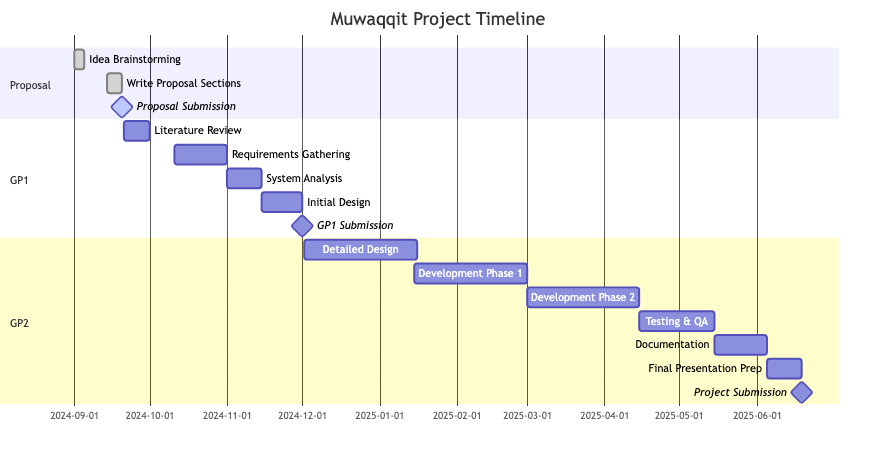
\includegraphics[width=\textwidth]{images/gantt.png}
    \caption{Project Gantt Chart}
    \label{fig:project-gantt-chart}
\end{figure}

\chapter{Literature Review}

In developing Muwaqqit, we have drawn inspiration from and built upon existing research and products in the field of intelligent calendar management. Some key references include:

\begin{itemize}
    \item \textbf{Clockwise (https://www.getclockwise.com/):} A smart calendar assistant that optimizes schedules and manages team coordination \cite{clockwise}. Clockwise's approach to intelligent time blocking and meeting optimization provides valuable insights for Muwaqqit's automated scheduling features.
    \item \textbf{Motion (https://www.usemotion.com/):} Motion's Intelligent Calendar takes your meetings, your tasks, your to-do list, your activities, and creates one perfect, optimized schedule to get it all done \cite{motion}.
    \item \textbf{Reclaim AI (https://reclaim.ai/):} An intelligent time management tool that helps optimize schedules and automate tasks \cite{reclaim}.
    \item \textbf{Calendi (https://calendi.ai/):} Calendi describes itself as: ``Calendi is an AI calendar system. Use it for scheduling tasks, automating meetings, and witness the future of calendar.'' \cite{calendi}
    \item \textbf{An Exploratory Study of Calendar Use:} ``Prospective remembering is the use of memory for remembering to do things in the future, as different from retrospective memory functions such as recalling past events.'' \cite{tungare2008exploratorystudycalendaruse}
    \item \textbf{WhatsApp Integration:} Our research indicates that direct WhatsApp integration for event extraction has not been widely implemented in existing calendar applications, making this a unique feature of Muwaqqit.
\end{itemize}

\begin{figure}[!h]
    \centering
    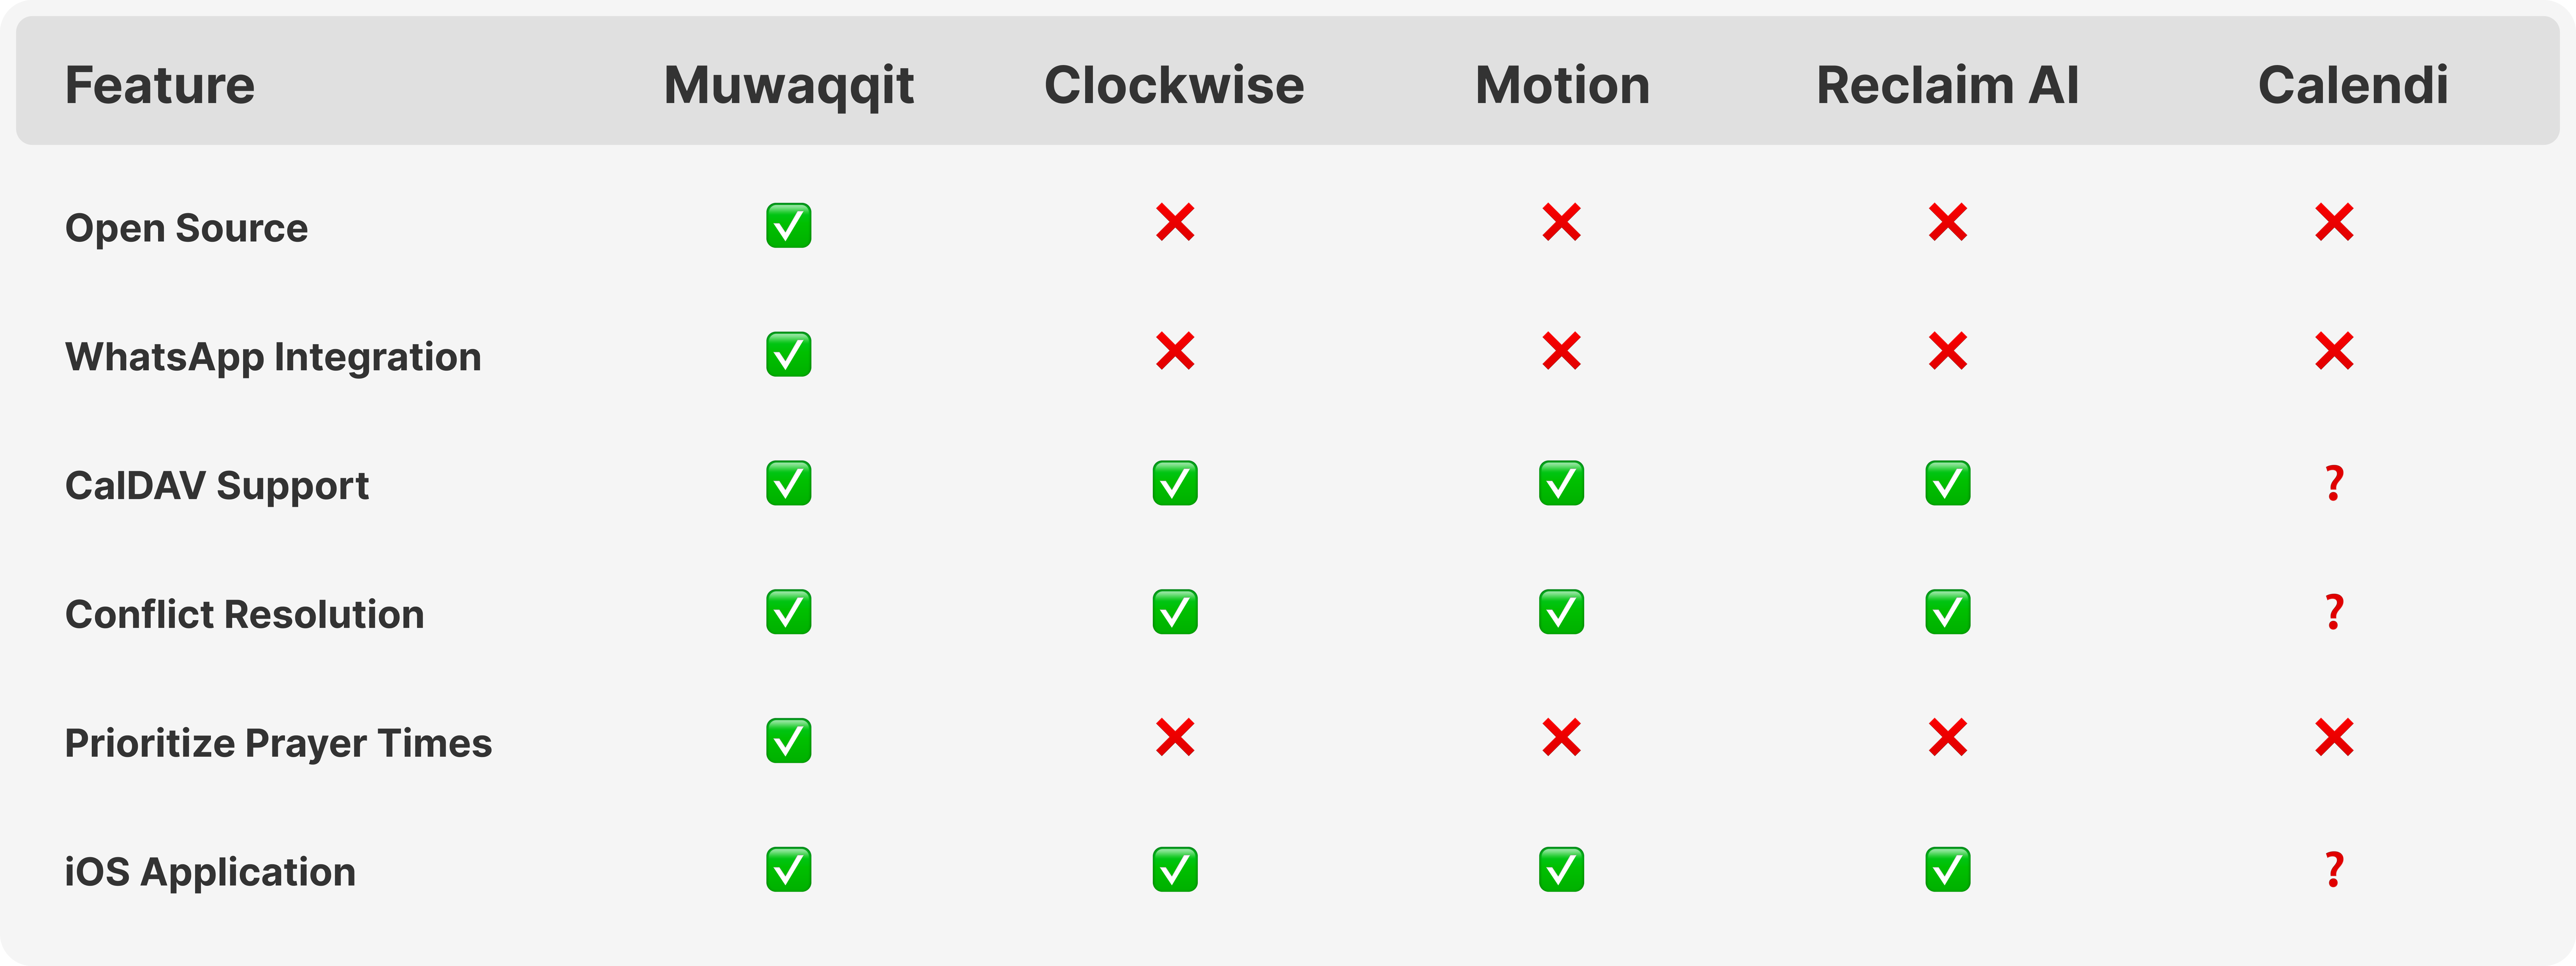
\includegraphics[width=\textwidth]{images/features-table.png}
    \caption{Feature Comparison Table}
    \label{fig:features-table}
\end{figure}

\chapter{System Analysis and Design}

% NEEDS WORK

\section{Functional Requirements}

\begin{itemize}
    \item The user shall be able to access their account using either Google OAuth or magic link via Email. For new users, a new accout is created, and for existing users, they are given access to their account directly
    \item The system shall send a welcome email to new users.
    \item The user should be able to connect a calendar using CalDAV.
    \item The user should be able to connect their WhatsApp account.
    \item The user should be able to add events manually and set priorities optionally.
    \item The user should be able to view integrated calendar.
    \item The user should be able to configure daily routines.
    \item The user should be able to manage scheduling conflicts.
    \item The user should be able to schedule prayer times.
    \item The system shall send event notifications to the user.
    \item The system shall personalize the experience based on answers provided by the users.
    \item The system shall add the WhatsApp extracted events to the calendar. If a conflict occurs, the user shall get a notification to resolve the conflict with suggestions.
    \item The system shall synchronize calendar data across multiple devices.
\end{itemize}

\section{Non-Functional Requirements}

\begin{itemize}
    \item \textbf{Platform Compatibility:} The app shall be compatible with iOS devices running iOS 14.0 or later.
    \item \textbf{Performance:} The app shall load the main calendar view within 3 seconds on 5G with speeds above 200mpbs.
    \item \textbf{User Experience:} The user interface shall follow iOS Human Interface Guidelines for consistency and ease of use.
    \item \textbf{Security:} All data transmissions between the app and servers shall be encrypted using HTTPS.
    \item \textbf{Localization:} The app shall support localization in Arabic and English.
    \item \textbf{Data Privacy:} The app shall comply with the data protection regulations and laws in Saudi Arabia.
\end{itemize}

\section{System use-cases}

\textbf{Figure \ref{fig:use-case-diagram}} shows the use case diagram for the system of Muwaqqit.

\begin{figure}[!h]
    \centering
    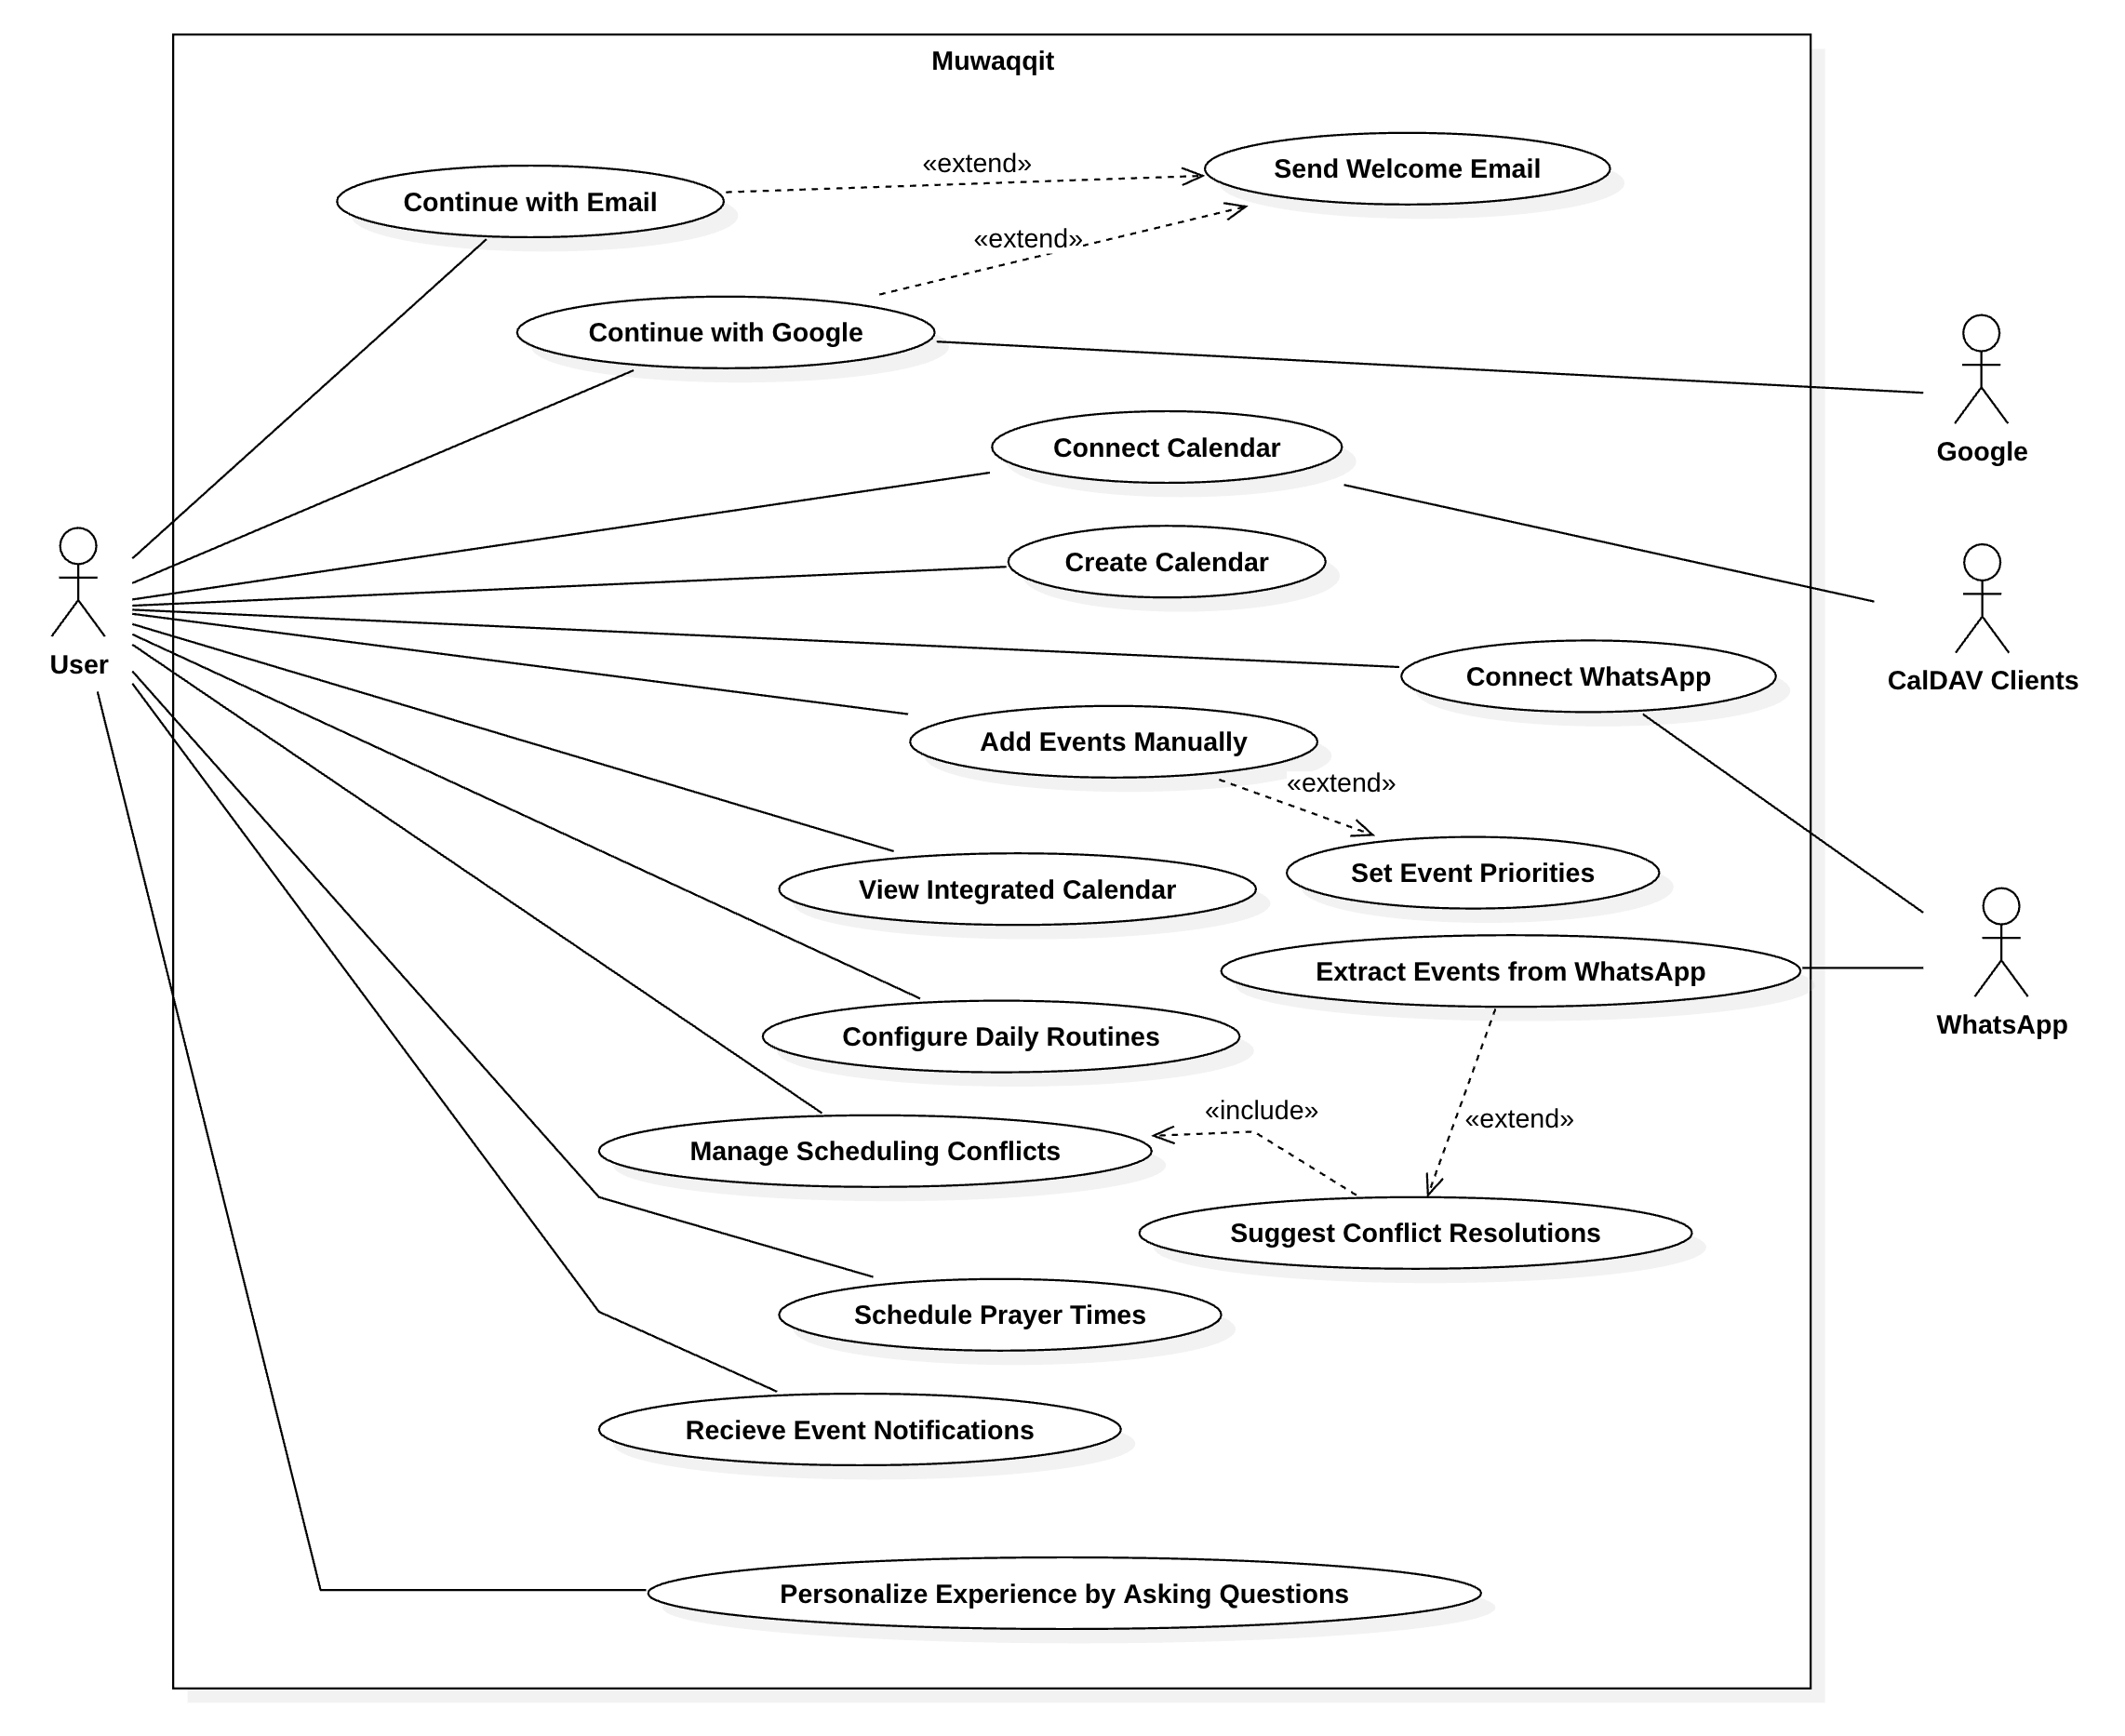
\includegraphics[width=\textwidth]{images/use-case-diagram.png}
    \caption{Use Case Diagram of Muwaqqit}
    \label{fig:use-case-diagram}
\end{figure}

% Bibliography
\bibliography{references}
\bibliographystyle{apalike}

\end{document}